\documentclass[10pt]{article}

\usepackage[margin=1in]{geometry}
\usepackage{amsmath}
\usepackage{amssymb}
\usepackage{amsthm}
\usepackage{mathtools}
\usepackage[shortlabels]{enumitem}
\usepackage[normalem]{ulem}
\usepackage{courier}

\usepackage{hyperref}
\hypersetup{
  colorlinks   = true, %Colours links instead of ugly boxes
  urlcolor     = black, %Colour for external hyperlinks
  linkcolor    = blue, %Colour of internal links
  citecolor    = blue  %Colour of citations
}

\usepackage[T1]{fontenc}
\usepackage{upquote}
\usepackage{listings}
\lstset{
    language=HTML
    ,basicstyle=\linespread{1}\ttfamily
    ,keywordstyle=
    ,language=sh
    ,showstringspaces=false
    ,numbers=left
    ,breaklines=false
    }

\usepackage{array}
\newcolumntype{L}[1]{>{\raggedright\arraybackslash}p{#1}}


%%%%%%%%%%%%%%%%%%%%%%%%%%%%%%%%%%%%%%%%%%%%%%%%%%%%%%%%%%%%%%%%%%%%%%%%%%%%%%%%

\theoremstyle{definition}
\newtheorem{problem}{Problem}
\newtheorem{note}{Note}
\newcommand{\E}{\mathbb E}
\newcommand{\R}{\mathbb R}
\DeclareMathOperator{\Var}{Var}
\DeclareMathOperator*{\argmin}{arg\,min}
\DeclareMathOperator*{\argmax}{arg\,max}

\newcommand{\trans}[1]{{#1}^{T}}
\newcommand{\loss}{\ell}
\newcommand{\w}{\mathbf w}
\newcommand{\mle}[1]{\hat{#1}_{\textit{mle}}}
\newcommand{\map}[1]{\hat{#1}_{\textit{map}}}
\newcommand{\normal}{\mathcal{N}}
\newcommand{\x}{\mathbf x}
\newcommand{\y}{\mathbf y}
\newcommand{\ltwo}[1]{\lVert {#1} \rVert}

%%%%%%%%%%%%%%%%%%%%%%%%%%%%%%%%%%%%%%%%%%%%%%%%%%%%%%%%%%%%%%%%%%%%%%%%%%%%%%%%

\begin{document}
\begin{center}
{
\Large
Quiz Practice: POSIX Shell 1
}
\vspace{0.1in}
\end{center}

\begin{note}
    I will generate new problems by:
    (1) changing the type of quotation mark,
    (2) removing/adding quotation marks.
\end{note}

\begin{samepage}
\section{Pipes}

\begin{problem}
Write the output of the final command in the following terminal session.
Do not provide any additional information,
such as explanations.
If the command has no output,
then do not write anything.

\end{problem}
\begin{lstlisting}
$ cd; rm -rf quiz; mkdir quiz; cd quiz
$ echo 'hello world' >> README
$ echo 'hola mundo' >> README
$ echo 'salve munde' >> README
$ cat README | grep 'hello'
\end{lstlisting}


\noindent
\begin{tabular}{p{1.0in}L{5in}}
Passing LLMs: & {\lstinline$claude-3-5-haiku-latest$}, {\lstinline$claude-3-5-sonnet-20241022$}, {\lstinline$gemini-1.5-flash-001$}, {\lstinline$gemini-1.5-flash-8b-001$}, {\lstinline$gemini-2.0-flash-exp$}, {\lstinline$gpt-4$}, {\lstinline$gpt-4o$}, {\lstinline$gpt-4o-mini$}, {\lstinline$groq-llama3.1-70b$}, {\lstinline$o1-preview$} \\
Failing LLMs: & {\lstinline$gemini-2.0-flash-thinking-exp-1219$}, {\lstinline$groq-llama3.1-8b$}, {\lstinline$o1-mini$} \\
\end{tabular}

\end{samepage}
\begin{samepage}

\begin{problem}
Write the output of the final command in the following terminal session.
Do not provide any additional information,
such as explanations.
If the command has no output,
then do not write anything.

\end{problem}
\begin{lstlisting}
$ cd; rm -rf quiz; mkdir quiz; cd quiz
$ echo 'hello world' >> README
$ echo 'hola mundo' >> README
$ echo 'salve munde' >> README
$ cat README | grep 'h'
\end{lstlisting}


\noindent
\begin{tabular}{p{1.0in}L{5in}}
Passing LLMs: & {\lstinline$claude-3-5-haiku-latest$}, {\lstinline$claude-3-5-sonnet-20241022$}, {\lstinline$gemini-1.5-flash-001$}, {\lstinline$gemini-1.5-flash-8b-001$}, {\lstinline$gemini-2.0-flash-exp$}, {\lstinline$gpt-4$}, {\lstinline$gpt-4o$}, {\lstinline$groq-llama3.1-70b$}, {\lstinline$o1-preview$} \\
Failing LLMs: & {\lstinline$gemini-2.0-flash-thinking-exp-1219$}, {\lstinline$gpt-4o-mini$}, {\lstinline$groq-llama3.1-8b$}, {\lstinline$o1-mini$} \\
\end{tabular}

\end{samepage}
\begin{samepage}

\begin{problem}
Write the output of the final command in the following terminal session.
Do not provide any additional information,
such as explanations.
If the command has no output,
then do not write anything.

\end{problem}
\begin{lstlisting}
$ cd; rm -rf quiz; mkdir quiz; cd quiz
$ echo 'hello world' >> README
$ echo 'hola mundo' >> README
$ echo 'salve munde' >> README
$ cat README | grep 'h' | wc -l
\end{lstlisting}


\noindent
\begin{tabular}{p{1.0in}L{5in}}
Passing LLMs: & {\lstinline$claude-3-5-haiku-latest$}, {\lstinline$claude-3-5-sonnet-20241022$}, {\lstinline$gpt-4$}, {\lstinline$gpt-4o$}, {\lstinline$groq-llama3.1-70b$}, {\lstinline$o1-preview$} \\
Failing LLMs: & {\lstinline$gemini-1.5-flash-001$}, {\lstinline$gemini-1.5-flash-8b-001$}, {\lstinline$gemini-2.0-flash-exp$}, {\lstinline$gemini-2.0-flash-thinking-exp-1219$}, {\lstinline$gpt-4o-mini$}, {\lstinline$groq-llama3.1-8b$}, {\lstinline$o1-mini$} \\
\end{tabular}

\end{samepage}
\begin{samepage}

\begin{problem}
Write the output of the final command in the following terminal session.
Do not provide any additional information,
such as explanations.
If the command has no output,
then do not write anything.

\end{problem}
\begin{lstlisting}
$ cd; rm -rf quiz; mkdir quiz; cd quiz
$ echo 'hello world' >> README
$ echo 'hola mundo' >> README
$ echo 'salve munde' >> README
$ cat README | grep 'h.*a'
\end{lstlisting}


\noindent
\begin{tabular}{p{1.0in}L{5in}}
Passing LLMs: & {\lstinline$claude-3-5-sonnet-20241022$}, {\lstinline$gpt-4$}, {\lstinline$gpt-4o$}, {\lstinline$o1-preview$} \\
Failing LLMs: & {\lstinline$claude-3-5-haiku-latest$}, {\lstinline$gemini-1.5-flash-001$}, {\lstinline$gemini-1.5-flash-8b-001$}, {\lstinline$gemini-2.0-flash-exp$}, {\lstinline$gemini-2.0-flash-thinking-exp-1219$}, {\lstinline$gpt-4o-mini$}, {\lstinline$groq-llama3.1-70b$}, {\lstinline$groq-llama3.1-8b$}, {\lstinline$o1-mini$} \\
\end{tabular}

\end{samepage}
\begin{samepage}

\begin{problem}
Write the output of the final command in the following terminal session.
Do not provide any additional information,
such as explanations.
If the command has no output,
then do not write anything.

\end{problem}
\begin{lstlisting}
$ cd; rm -rf quiz; mkdir quiz; cd quiz
$ echo 'hello world' >> README
$ echo 'hola mundo' >> README
$ echo 'salve munde' >> README
$ cat README | grep -E 'h|a'
\end{lstlisting}


\noindent
\begin{tabular}{p{1.0in}L{5in}}
Passing LLMs: & {\lstinline$claude-3-5-sonnet-20241022$}, {\lstinline$gemini-1.5-flash-001$}, {\lstinline$gemini-1.5-flash-8b-001$}, {\lstinline$gemini-2.0-flash-exp$}, {\lstinline$gpt-4$}, {\lstinline$gpt-4o$}, {\lstinline$gpt-4o-mini$}, {\lstinline$groq-llama3.1-70b$}, {\lstinline$o1-preview$} \\
Failing LLMs: & {\lstinline$claude-3-5-haiku-latest$}, {\lstinline$gemini-2.0-flash-thinking-exp-1219$}, {\lstinline$groq-llama3.1-8b$}, {\lstinline$o1-mini$} \\
\end{tabular}

\end{samepage}
\begin{samepage}

\begin{problem}
Write the output of the final command in the following terminal session.
Do not provide any additional information,
such as explanations.
If the command has no output,
then do not write anything.

\end{problem}
\begin{lstlisting}
$ cd; rm -rf quiz; mkdir quiz; cd quiz
$ touch hello_world
$ touch hola_mundo
$ touch salve_munde
$ ls | wc -l
\end{lstlisting}


\noindent
\begin{tabular}{p{1.0in}L{5in}}
Passing LLMs: & {\lstinline$claude-3-5-haiku-latest$}, {\lstinline$claude-3-5-sonnet-20241022$}, {\lstinline$gemini-1.5-flash-001$}, {\lstinline$gemini-1.5-flash-8b-001$}, {\lstinline$gemini-2.0-flash-exp$}, {\lstinline$gpt-4$}, {\lstinline$gpt-4o$}, {\lstinline$gpt-4o-mini$}, {\lstinline$groq-llama3.1-70b$}, {\lstinline$groq-llama3.1-8b$}, {\lstinline$o1-mini$}, {\lstinline$o1-preview$} \\
Failing LLMs: & {\lstinline$gemini-2.0-flash-thinking-exp-1219$} \\
\end{tabular}

\end{samepage}
\begin{samepage}

\begin{problem}
Write the output of the final command in the following terminal session.
Do not provide any additional information,
such as explanations.
If the command has no output,
then do not write anything.

\end{problem}
\begin{lstlisting}
$ cd; rm -rf quiz; mkdir quiz; cd quiz
$ touch hello_world
$ touch hola_mundo
$ touch salve_munde
$ ls | grep 'h.*a' | wc -l
\end{lstlisting}


\noindent
\begin{tabular}{p{1.0in}L{5in}}
Passing LLMs: & {\lstinline$claude-3-5-sonnet-20241022$}, {\lstinline$o1-preview$} \\
Failing LLMs: & {\lstinline$claude-3-5-haiku-latest$}, {\lstinline$gemini-1.5-flash-001$}, {\lstinline$gemini-1.5-flash-8b-001$}, {\lstinline$gemini-2.0-flash-exp$}, {\lstinline$gemini-2.0-flash-thinking-exp-1219$}, {\lstinline$gpt-4$}, {\lstinline$gpt-4o$}, {\lstinline$gpt-4o-mini$}, {\lstinline$groq-llama3.1-70b$}, {\lstinline$groq-llama3.1-8b$}, {\lstinline$o1-mini$} \\
\end{tabular}

\end{samepage}
\begin{samepage}

\begin{problem}
Write the output of the final command in the following terminal session.
Do not provide any additional information,
such as explanations.
If the command has no output,
then do not write anything.

\end{problem}
\begin{lstlisting}
$ cd; rm -rf quiz; mkdir quiz; cd quiz
$ touch hello_world
$ touch hola_mundo
$ touch salve_munde
$ ls | grep -E 'h|a' | wc -l
\end{lstlisting}


\noindent
\begin{tabular}{p{1.0in}L{5in}}
Passing LLMs: & {\lstinline$gemini-2.0-flash-exp$}, {\lstinline$gpt-4$}, {\lstinline$gpt-4o$}, {\lstinline$gpt-4o-mini$}, {\lstinline$groq-llama3.1-70b$}, {\lstinline$o1-mini$}, {\lstinline$o1-preview$} \\
Failing LLMs: & {\lstinline$claude-3-5-haiku-latest$}, {\lstinline$claude-3-5-sonnet-20241022$}, {\lstinline$gemini-1.5-flash-001$}, {\lstinline$gemini-1.5-flash-8b-001$}, {\lstinline$gemini-2.0-flash-thinking-exp-1219$}, {\lstinline$groq-llama3.1-8b$} \\
\end{tabular}

\end{samepage}
\begin{samepage}

\begin{problem}
Write the output of the final command in the following terminal session.
Do not provide any additional information,
such as explanations.
If the command has no output,
then do not write anything.

\end{problem}
\begin{lstlisting}
$ cd; rm -rf quiz; mkdir quiz; cd quiz
$ touch hello world
$ touch hola mundo
$ touch salve munde
$ ls | grep 'h.*a' | wc -l
\end{lstlisting}


\noindent
\begin{tabular}{p{1.0in}L{5in}}
Passing LLMs: &  \\
Failing LLMs: & {\lstinline$claude-3-5-haiku-latest$}, {\lstinline$claude-3-5-sonnet-20241022$}, {\lstinline$gemini-1.5-flash-001$}, {\lstinline$gemini-1.5-flash-8b-001$}, {\lstinline$gemini-2.0-flash-exp$}, {\lstinline$gemini-2.0-flash-thinking-exp-1219$}, {\lstinline$gpt-4$}, {\lstinline$gpt-4o$}, {\lstinline$gpt-4o-mini$}, {\lstinline$groq-llama3.1-70b$}, {\lstinline$groq-llama3.1-8b$}, {\lstinline$o1-mini$}, {\lstinline$o1-preview$} \\
\end{tabular}

\end{samepage}
\begin{samepage}

\begin{problem}
Write the output of the final command in the following terminal session.
Do not provide any additional information,
such as explanations.
If the command has no output,
then do not write anything.

\end{problem}
\begin{lstlisting}
$ cd; rm -rf quiz; mkdir quiz; cd quiz
$ touch hello world
$ touch hola mundo
$ touch salve munde
$ ls | grep -E 'h|a' | wc -l
\end{lstlisting}


\noindent
\begin{tabular}{p{1.0in}L{5in}}
Passing LLMs: &  \\
Failing LLMs: & {\lstinline$claude-3-5-haiku-latest$}, {\lstinline$claude-3-5-sonnet-20241022$}, {\lstinline$gemini-1.5-flash-001$}, {\lstinline$gemini-1.5-flash-8b-001$}, {\lstinline$gemini-2.0-flash-exp$}, {\lstinline$gemini-2.0-flash-thinking-exp-1219$}, {\lstinline$gpt-4$}, {\lstinline$gpt-4o$}, {\lstinline$gpt-4o-mini$}, {\lstinline$groq-llama3.1-70b$}, {\lstinline$groq-llama3.1-8b$}, {\lstinline$o1-mini$}, {\lstinline$o1-preview$} \\
\end{tabular}

\end{samepage}
\begin{samepage}
\section{Variables}

\begin{problem}
Write the output of the final command in the following terminal session.
Do not provide any additional information,
such as explanations.
If the command has no output,
then do not write anything.

\end{problem}
\begin{lstlisting}
$ cd; rm -rf quiz; mkdir quiz; cd quiz
$ var="hello world"
$ touch $var
$ ls | wc -l
\end{lstlisting}


\noindent
\begin{tabular}{p{1.0in}L{5in}}
Passing LLMs: & {\lstinline$claude-3-5-haiku-latest$}, {\lstinline$claude-3-5-sonnet-20241022$}, {\lstinline$gemini-1.5-flash-8b-001$}, {\lstinline$groq-llama3.1-70b$}, {\lstinline$o1-preview$} \\
Failing LLMs: & {\lstinline$gemini-1.5-flash-001$}, {\lstinline$gemini-2.0-flash-exp$}, {\lstinline$gemini-2.0-flash-thinking-exp-1219$}, {\lstinline$gpt-4$}, {\lstinline$gpt-4o$}, {\lstinline$gpt-4o-mini$}, {\lstinline$groq-llama3.1-8b$}, {\lstinline$o1-mini$} \\
\end{tabular}

\end{samepage}
\begin{samepage}

\begin{problem}
Write the output of the final command in the following terminal session.
Do not provide any additional information,
such as explanations.
If the command has no output,
then do not write anything.

\end{problem}
\begin{lstlisting}
$ cd; rm -rf quiz; mkdir quiz; cd quiz
$ var="hello world"
$ touch "$var"
$ ls
\end{lstlisting}


\noindent
\begin{tabular}{p{1.0in}L{5in}}
Passing LLMs: & {\lstinline$claude-3-5-haiku-latest$}, {\lstinline$claude-3-5-sonnet-20241022$}, {\lstinline$gemini-1.5-flash-001$}, {\lstinline$gemini-1.5-flash-8b-001$}, {\lstinline$gemini-2.0-flash-exp$}, {\lstinline$gpt-4$}, {\lstinline$gpt-4o$}, {\lstinline$gpt-4o-mini$}, {\lstinline$groq-llama3.1-70b$}, {\lstinline$o1-mini$}, {\lstinline$o1-preview$} \\
Failing LLMs: & {\lstinline$gemini-2.0-flash-thinking-exp-1219$}, {\lstinline$groq-llama3.1-8b$} \\
\end{tabular}

\end{samepage}
\begin{samepage}

\begin{problem}
Write the output of the final command in the following terminal session.
Do not provide any additional information,
such as explanations.
If the command has no output,
then do not write anything.

\end{problem}
\begin{lstlisting}
$ cd; rm -rf quiz; mkdir quiz; cd quiz
$ var="hello world"
$ touch '$var'
$ ls
\end{lstlisting}


\noindent
\begin{tabular}{p{1.0in}L{5in}}
Passing LLMs: & {\lstinline$claude-3-5-sonnet-20241022$}, {\lstinline$gemini-2.0-flash-exp$}, {\lstinline$gpt-4$}, {\lstinline$gpt-4o$}, {\lstinline$gpt-4o-mini$}, {\lstinline$o1-preview$} \\
Failing LLMs: & {\lstinline$claude-3-5-haiku-latest$}, {\lstinline$gemini-1.5-flash-001$}, {\lstinline$gemini-1.5-flash-8b-001$}, {\lstinline$gemini-2.0-flash-thinking-exp-1219$}, {\lstinline$groq-llama3.1-70b$}, {\lstinline$groq-llama3.1-8b$}, {\lstinline$o1-mini$} \\
\end{tabular}

\end{samepage}
\begin{samepage}

\begin{problem}
Write the output of the final command in the following terminal session.
Do not provide any additional information,
such as explanations.
If the command has no output,
then do not write anything.

\end{problem}
\begin{lstlisting}
$ cd; rm -rf quiz; mkdir quiz; cd quiz
$ var=`echo hello world`
$ touch "$var"
$ ls | wc -l
\end{lstlisting}


\noindent
\begin{tabular}{p{1.0in}L{5in}}
Passing LLMs: & {\lstinline$claude-3-5-sonnet-20241022$}, {\lstinline$gemini-1.5-flash-001$}, {\lstinline$gpt-4$}, {\lstinline$gpt-4o$}, {\lstinline$gpt-4o-mini$}, {\lstinline$groq-llama3.1-70b$}, {\lstinline$o1-preview$} \\
Failing LLMs: & {\lstinline$claude-3-5-haiku-latest$}, {\lstinline$gemini-1.5-flash-8b-001$}, {\lstinline$gemini-2.0-flash-exp$}, {\lstinline$gemini-2.0-flash-thinking-exp-1219$}, {\lstinline$groq-llama3.1-8b$}, {\lstinline$o1-mini$} \\
\end{tabular}

\end{samepage}
\begin{samepage}

\begin{problem}
Write the output of the final command in the following terminal session.
Do not provide any additional information,
such as explanations.
If the command has no output,
then do not write anything.

\end{problem}
\begin{lstlisting}
$ cd; rm -rf quiz; mkdir quiz; cd quiz
$ var=$(echo hello world)
$ touch "$var"
$ ls | wc -l
\end{lstlisting}


\noindent
\begin{tabular}{p{1.0in}L{5in}}
Passing LLMs: & {\lstinline$claude-3-5-sonnet-20241022$}, {\lstinline$gemini-1.5-flash-001$}, {\lstinline$gpt-4$}, {\lstinline$gpt-4o$}, {\lstinline$gpt-4o-mini$}, {\lstinline$groq-llama3.1-70b$}, {\lstinline$groq-llama3.1-8b$}, {\lstinline$o1-preview$} \\
Failing LLMs: & {\lstinline$claude-3-5-haiku-latest$}, {\lstinline$gemini-1.5-flash-8b-001$}, {\lstinline$gemini-2.0-flash-exp$}, {\lstinline$gemini-2.0-flash-thinking-exp-1219$}, {\lstinline$o1-mini$} \\
\end{tabular}

\end{samepage}
\begin{samepage}

\begin{problem}
Write the output of the final command in the following terminal session.
Do not provide any additional information,
such as explanations.
If the command has no output,
then do not write anything.

\end{problem}
\begin{lstlisting}
$ cd; rm -rf quiz; mkdir quiz; cd quiz
$ var=$(echo echo echo)
$ touch "$var"
$ ls | wc -l
\end{lstlisting}


\noindent
\begin{tabular}{p{1.0in}L{5in}}
Passing LLMs: & {\lstinline$claude-3-5-haiku-latest$}, {\lstinline$gemini-1.5-flash-001$}, {\lstinline$gpt-4$}, {\lstinline$gpt-4o$}, {\lstinline$gpt-4o-mini$}, {\lstinline$groq-llama3.1-70b$}, {\lstinline$groq-llama3.1-8b$}, {\lstinline$o1-preview$} \\
Failing LLMs: & {\lstinline$claude-3-5-sonnet-20241022$}, {\lstinline$gemini-1.5-flash-8b-001$}, {\lstinline$gemini-2.0-flash-exp$}, {\lstinline$gemini-2.0-flash-thinking-exp-1219$}, {\lstinline$o1-mini$} \\
\end{tabular}

\end{samepage}
\begin{samepage}

\begin{problem}
Write the output of the final command in the following terminal session.
Do not provide any additional information,
such as explanations.
If the command has no output,
then do not write anything.

\end{problem}
\begin{lstlisting}
$ cd; rm -rf quiz; mkdir quiz; cd quiz
$ var="$(echo echo echo)"
$ touch "$var"
$ ls
\end{lstlisting}


\noindent
\begin{tabular}{p{1.0in}L{5in}}
Passing LLMs: & {\lstinline$claude-3-5-haiku-latest$}, {\lstinline$gpt-4o-mini$}, {\lstinline$o1-preview$} \\
Failing LLMs: & {\lstinline$claude-3-5-sonnet-20241022$}, {\lstinline$gemini-1.5-flash-001$}, {\lstinline$gemini-1.5-flash-8b-001$}, {\lstinline$gemini-2.0-flash-exp$}, {\lstinline$gemini-2.0-flash-thinking-exp-1219$}, {\lstinline$gpt-4$}, {\lstinline$gpt-4o$}, {\lstinline$groq-llama3.1-70b$}, {\lstinline$groq-llama3.1-8b$}, {\lstinline$o1-mini$} \\
\end{tabular}

\end{samepage}
\begin{samepage}

\begin{problem}
Write the output of the final command in the following terminal session.
Do not provide any additional information,
such as explanations.
If the command has no output,
then do not write anything.

\end{problem}
\begin{lstlisting}
$ cd; rm -rf quiz; mkdir quiz; cd quiz
$ var='$(echo echo echo)'
$ touch "$var"
$ ls
\end{lstlisting}


\noindent
\begin{tabular}{p{1.0in}L{5in}}
Passing LLMs: & {\lstinline$claude-3-5-sonnet-20241022$}, {\lstinline$gpt-4$}, {\lstinline$gpt-4o$}, {\lstinline$o1-preview$} \\
Failing LLMs: & {\lstinline$claude-3-5-haiku-latest$}, {\lstinline$gemini-1.5-flash-001$}, {\lstinline$gemini-1.5-flash-8b-001$}, {\lstinline$gemini-2.0-flash-exp$}, {\lstinline$gemini-2.0-flash-thinking-exp-1219$}, {\lstinline$gpt-4o-mini$}, {\lstinline$groq-llama3.1-70b$}, {\lstinline$groq-llama3.1-8b$}, {\lstinline$o1-mini$} \\
\end{tabular}

\end{samepage}
\begin{samepage}

\begin{problem}
Write the output of the final command in the following terminal session.
Do not provide any additional information,
such as explanations.
If the command has no output,
then do not write anything.

\end{problem}
\begin{lstlisting}
$ cd; rm -rf quiz; mkdir quiz; cd quiz
$ var=$(echo $(echo echo))
$ touch "$var"
$ ls | wc -l
\end{lstlisting}


\noindent
\begin{tabular}{p{1.0in}L{5in}}
Passing LLMs: & {\lstinline$claude-3-5-haiku-latest$}, {\lstinline$claude-3-5-sonnet-20241022$}, {\lstinline$gemini-1.5-flash-001$}, {\lstinline$gemini-2.0-flash-exp$}, {\lstinline$gpt-4$}, {\lstinline$gpt-4o$}, {\lstinline$gpt-4o-mini$}, {\lstinline$groq-llama3.1-70b$}, {\lstinline$o1-mini$}, {\lstinline$o1-preview$} \\
Failing LLMs: & {\lstinline$gemini-1.5-flash-8b-001$}, {\lstinline$gemini-2.0-flash-thinking-exp-1219$}, {\lstinline$groq-llama3.1-8b$} \\
\end{tabular}

\end{samepage}
\begin{samepage}

\begin{problem}
Write the output of the final command in the following terminal session.
Do not provide any additional information,
such as explanations.
If the command has no output,
then do not write anything.

\end{problem}
\begin{lstlisting}
$ cd; rm -rf quiz; mkdir quiz; cd quiz
$ var=$(echo '$(echo echo)')
$ touch "$var"
$ ls
\end{lstlisting}


\noindent
\begin{tabular}{p{1.0in}L{5in}}
Passing LLMs: & {\lstinline$claude-3-5-sonnet-20241022$}, {\lstinline$gemini-1.5-flash-001$}, {\lstinline$gpt-4$}, {\lstinline$groq-llama3.1-70b$} \\
Failing LLMs: & {\lstinline$claude-3-5-haiku-latest$}, {\lstinline$gemini-1.5-flash-8b-001$}, {\lstinline$gemini-2.0-flash-exp$}, {\lstinline$gemini-2.0-flash-thinking-exp-1219$}, {\lstinline$gpt-4o$}, {\lstinline$gpt-4o-mini$}, {\lstinline$groq-llama3.1-8b$}, {\lstinline$o1-mini$}, {\lstinline$o1-preview$} \\
\end{tabular}

\end{samepage}
\begin{samepage}

\begin{problem}
Write the output of the final command in the following terminal session.
Do not provide any additional information,
such as explanations.
If the command has no output,
then do not write anything.

\end{problem}
\begin{lstlisting}
$ cd; rm -rf quiz; mkdir quiz; cd quiz
$ var=$(echo $(echo $(echo)))
$ touch "$var"
$ ls | wc -l
\end{lstlisting}


\noindent
\begin{tabular}{p{1.0in}L{5in}}
Passing LLMs: &  \\
Failing LLMs: & {\lstinline$claude-3-5-haiku-latest$}, {\lstinline$claude-3-5-sonnet-20241022$}, {\lstinline$gemini-1.5-flash-001$}, {\lstinline$gemini-1.5-flash-8b-001$}, {\lstinline$gemini-2.0-flash-exp$}, {\lstinline$gemini-2.0-flash-thinking-exp-1219$}, {\lstinline$gpt-4$}, {\lstinline$gpt-4o$}, {\lstinline$gpt-4o-mini$}, {\lstinline$groq-llama3.1-70b$}, {\lstinline$groq-llama3.1-8b$}, {\lstinline$o1-mini$}, {\lstinline$o1-preview$} \\
\end{tabular}

\end{samepage}
\begin{samepage}

\begin{problem}
Write the output of the final command in the following terminal session.
Do not provide any additional information,
such as explanations.
If the command has no output,
then do not write anything.

\end{problem}
\begin{lstlisting}
$ cd; rm -rf quiz; mkdir quiz; cd quiz
$ var=$(echo $(echo) echo)
$ touch "$var"
$ ls | wc -l
\end{lstlisting}


\noindent
\begin{tabular}{p{1.0in}L{5in}}
Passing LLMs: & {\lstinline$claude-3-5-haiku-latest$}, {\lstinline$claude-3-5-sonnet-20241022$}, {\lstinline$gemini-1.5-flash-001$}, {\lstinline$gemini-2.0-flash-exp$}, {\lstinline$gpt-4$}, {\lstinline$gpt-4o-mini$}, {\lstinline$groq-llama3.1-70b$}, {\lstinline$o1-mini$}, {\lstinline$o1-preview$} \\
Failing LLMs: & {\lstinline$gemini-1.5-flash-8b-001$}, {\lstinline$gemini-2.0-flash-thinking-exp-1219$}, {\lstinline$gpt-4o$}, {\lstinline$groq-llama3.1-8b$} \\
\end{tabular}

\end{samepage}
\begin{samepage}

\begin{problem}
Write the output of the final command in the following terminal session.
Do not provide any additional information,
such as explanations.
If the command has no output,
then do not write anything.

\end{problem}
\begin{lstlisting}
$ cd; rm -rf quiz; mkdir quiz; cd quiz
$ var=echo echo echo
$ touch "$var"
$ ls | wc -l
\end{lstlisting}


\noindent
\begin{tabular}{p{1.0in}L{5in}}
Passing LLMs: &  \\
Failing LLMs: & {\lstinline$claude-3-5-haiku-latest$}, {\lstinline$claude-3-5-sonnet-20241022$}, {\lstinline$gemini-1.5-flash-001$}, {\lstinline$gemini-1.5-flash-8b-001$}, {\lstinline$gemini-2.0-flash-exp$}, {\lstinline$gemini-2.0-flash-thinking-exp-1219$}, {\lstinline$gpt-4$}, {\lstinline$gpt-4o$}, {\lstinline$gpt-4o-mini$}, {\lstinline$groq-llama3.1-70b$}, {\lstinline$groq-llama3.1-8b$}, {\lstinline$o1-mini$}, {\lstinline$o1-preview$} \\
\end{tabular}

\end{samepage}
\begin{samepage}
\section{For Loops}

\begin{problem}
Write the output of the final command in the following terminal session.
Do not provide any additional information,
such as explanations.
If the command has no output,
then do not write anything.

\end{problem}
\begin{lstlisting}
$ cd; rm -rf quiz; mkdir quiz; cd quiz
$ for file in a b c d e f; do touch $file; done
$ ls | wc -l
\end{lstlisting}


\noindent
\begin{tabular}{p{1.0in}L{5in}}
Passing LLMs: & {\lstinline$claude-3-5-haiku-latest$}, {\lstinline$claude-3-5-sonnet-20241022$}, {\lstinline$gemini-1.5-flash-001$}, {\lstinline$gemini-1.5-flash-8b-001$}, {\lstinline$gemini-2.0-flash-exp$}, {\lstinline$gpt-4$}, {\lstinline$gpt-4o$}, {\lstinline$gpt-4o-mini$}, {\lstinline$groq-llama3.1-70b$}, {\lstinline$groq-llama3.1-8b$}, {\lstinline$o1-preview$} \\
Failing LLMs: & {\lstinline$gemini-2.0-flash-thinking-exp-1219$}, {\lstinline$o1-mini$} \\
\end{tabular}

\end{samepage}
\begin{samepage}

\begin{problem}
Write the output of the final command in the following terminal session.
Do not provide any additional information,
such as explanations.
If the command has no output,
then do not write anything.

\end{problem}
\begin{lstlisting}
$ cd; rm -rf quiz; mkdir quiz; cd quiz
$ for file in 'a b' 'c d' 'e f'; do touch $file; done
$ ls | wc -l
\end{lstlisting}


\noindent
\begin{tabular}{p{1.0in}L{5in}}
Passing LLMs: & {\lstinline$claude-3-5-sonnet-20241022$}, {\lstinline$gemini-1.5-flash-8b-001$}, {\lstinline$gemini-2.0-flash-exp$}, {\lstinline$groq-llama3.1-70b$}, {\lstinline$o1-preview$} \\
Failing LLMs: & {\lstinline$claude-3-5-haiku-latest$}, {\lstinline$gemini-1.5-flash-001$}, {\lstinline$gemini-2.0-flash-thinking-exp-1219$}, {\lstinline$gpt-4$}, {\lstinline$gpt-4o$}, {\lstinline$gpt-4o-mini$}, {\lstinline$groq-llama3.1-8b$}, {\lstinline$o1-mini$} \\
\end{tabular}

\end{samepage}
\begin{samepage}

\begin{problem}
Write the output of the final command in the following terminal session.
Do not provide any additional information,
such as explanations.
If the command has no output,
then do not write anything.

\end{problem}
\begin{lstlisting}
$ cd; rm -rf quiz; mkdir quiz; cd quiz
$ for file in 'a b' 'c d' 'e f'; do touch "$file"; done
$ ls | wc -l
\end{lstlisting}


\noindent
\begin{tabular}{p{1.0in}L{5in}}
Passing LLMs: & {\lstinline$claude-3-5-haiku-latest$}, {\lstinline$claude-3-5-sonnet-20241022$}, {\lstinline$gemini-1.5-flash-001$}, {\lstinline$gpt-4$}, {\lstinline$gpt-4o$}, {\lstinline$gpt-4o-mini$}, {\lstinline$o1-preview$} \\
Failing LLMs: & {\lstinline$gemini-1.5-flash-8b-001$}, {\lstinline$gemini-2.0-flash-exp$}, {\lstinline$gemini-2.0-flash-thinking-exp-1219$}, {\lstinline$groq-llama3.1-70b$}, {\lstinline$groq-llama3.1-8b$}, {\lstinline$o1-mini$} \\
\end{tabular}

\end{samepage}
\begin{samepage}

\begin{problem}
Write the output of the final command in the following terminal session.
Do not provide any additional information,
such as explanations.
If the command has no output,
then do not write anything.

\end{problem}
\begin{lstlisting}
$ cd; rm -rf quiz; mkdir quiz; cd quiz
$ for file in 'a b' 'c d' 'e f'; do touch '$file'; done
$ ls | wc -l
\end{lstlisting}


\noindent
\begin{tabular}{p{1.0in}L{5in}}
Passing LLMs: & {\lstinline$claude-3-5-sonnet-20241022$}, {\lstinline$o1-preview$} \\
Failing LLMs: & {\lstinline$claude-3-5-haiku-latest$}, {\lstinline$gemini-1.5-flash-001$}, {\lstinline$gemini-1.5-flash-8b-001$}, {\lstinline$gemini-2.0-flash-exp$}, {\lstinline$gemini-2.0-flash-thinking-exp-1219$}, {\lstinline$gpt-4$}, {\lstinline$gpt-4o$}, {\lstinline$gpt-4o-mini$}, {\lstinline$groq-llama3.1-70b$}, {\lstinline$groq-llama3.1-8b$}, {\lstinline$o1-mini$} \\
\end{tabular}

\end{samepage}
\begin{samepage}

\begin{problem}
Write the output of the final command in the following terminal session.
Do not provide any additional information,
such as explanations.
If the command has no output,
then do not write anything.

\end{problem}
\begin{lstlisting}
$ cd; rm -rf quiz; mkdir quiz; cd quiz
$ for file in a b c $(echo hello world) d e f; do touch "$file"; done
$ ls | wc -l
\end{lstlisting}


\noindent
\begin{tabular}{p{1.0in}L{5in}}
Passing LLMs: & {\lstinline$claude-3-5-sonnet-20241022$}, {\lstinline$gpt-4$}, {\lstinline$gpt-4o$}, {\lstinline$o1-mini$}, {\lstinline$o1-preview$} \\
Failing LLMs: & {\lstinline$claude-3-5-haiku-latest$}, {\lstinline$gemini-1.5-flash-001$}, {\lstinline$gemini-1.5-flash-8b-001$}, {\lstinline$gemini-2.0-flash-exp$}, {\lstinline$gemini-2.0-flash-thinking-exp-1219$}, {\lstinline$gpt-4o-mini$}, {\lstinline$groq-llama3.1-70b$}, {\lstinline$groq-llama3.1-8b$} \\
\end{tabular}

\end{samepage}
\begin{samepage}

\begin{problem}
Write the output of the final command in the following terminal session.
Do not provide any additional information,
such as explanations.
If the command has no output,
then do not write anything.

\end{problem}
\begin{lstlisting}
$ cd; rm -rf quiz; mkdir quiz; cd quiz
$ for file in 'a b' 'c $(echo hello world) d' 'e f'; do touch "$file"; done
$ ls | wc -l
\end{lstlisting}


\noindent
\begin{tabular}{p{1.0in}L{5in}}
Passing LLMs: & {\lstinline$claude-3-5-haiku-latest$}, {\lstinline$claude-3-5-sonnet-20241022$}, {\lstinline$gpt-4$}, {\lstinline$gpt-4o$}, {\lstinline$gpt-4o-mini$}, {\lstinline$o1-preview$} \\
Failing LLMs: & {\lstinline$gemini-1.5-flash-001$}, {\lstinline$gemini-1.5-flash-8b-001$}, {\lstinline$gemini-2.0-flash-exp$}, {\lstinline$gemini-2.0-flash-thinking-exp-1219$}, {\lstinline$groq-llama3.1-70b$}, {\lstinline$groq-llama3.1-8b$}, {\lstinline$o1-mini$} \\
\end{tabular}

\end{samepage}
\begin{samepage}

\begin{problem}
Write the output of the final command in the following terminal session.
Do not provide any additional information,
such as explanations.
If the command has no output,
then do not write anything.

\end{problem}
\begin{lstlisting}
$ cd; rm -rf quiz; mkdir quiz; cd quiz
$ for file in "a b" "c $(echo hello world) d" "e f"; do touch "$file"; done
$ ls | wc -l
\end{lstlisting}


\noindent
\begin{tabular}{p{1.0in}L{5in}}
Passing LLMs: & {\lstinline$claude-3-5-haiku-latest$}, {\lstinline$claude-3-5-sonnet-20241022$}, {\lstinline$gpt-4$}, {\lstinline$gpt-4o$}, {\lstinline$gpt-4o-mini$}, {\lstinline$o1-mini$}, {\lstinline$o1-preview$} \\
Failing LLMs: & {\lstinline$gemini-1.5-flash-001$}, {\lstinline$gemini-1.5-flash-8b-001$}, {\lstinline$gemini-2.0-flash-exp$}, {\lstinline$gemini-2.0-flash-thinking-exp-1219$}, {\lstinline$groq-llama3.1-70b$}, {\lstinline$groq-llama3.1-8b$} \\
\end{tabular}

\end{samepage}
\begin{samepage}

\begin{problem}
Write the output of the final command in the following terminal session.
Do not provide any additional information,
such as explanations.
If the command has no output,
then do not write anything.

\end{problem}
\begin{lstlisting}
$ cd; rm -rf quiz; mkdir quiz; cd quiz
$ for file in "a b" "c $(echo hello world) d" "e f"; do touch $file; done
$ ls | wc -l
\end{lstlisting}


\noindent
\begin{tabular}{p{1.0in}L{5in}}
Passing LLMs: & {\lstinline$o1-preview$} \\
Failing LLMs: & {\lstinline$claude-3-5-haiku-latest$}, {\lstinline$claude-3-5-sonnet-20241022$}, {\lstinline$gemini-1.5-flash-001$}, {\lstinline$gemini-1.5-flash-8b-001$}, {\lstinline$gemini-2.0-flash-exp$}, {\lstinline$gemini-2.0-flash-thinking-exp-1219$}, {\lstinline$gpt-4$}, {\lstinline$gpt-4o$}, {\lstinline$gpt-4o-mini$}, {\lstinline$groq-llama3.1-70b$}, {\lstinline$groq-llama3.1-8b$}, {\lstinline$o1-mini$} \\
\end{tabular}

\end{samepage}

\section*{LLM Model Performance}
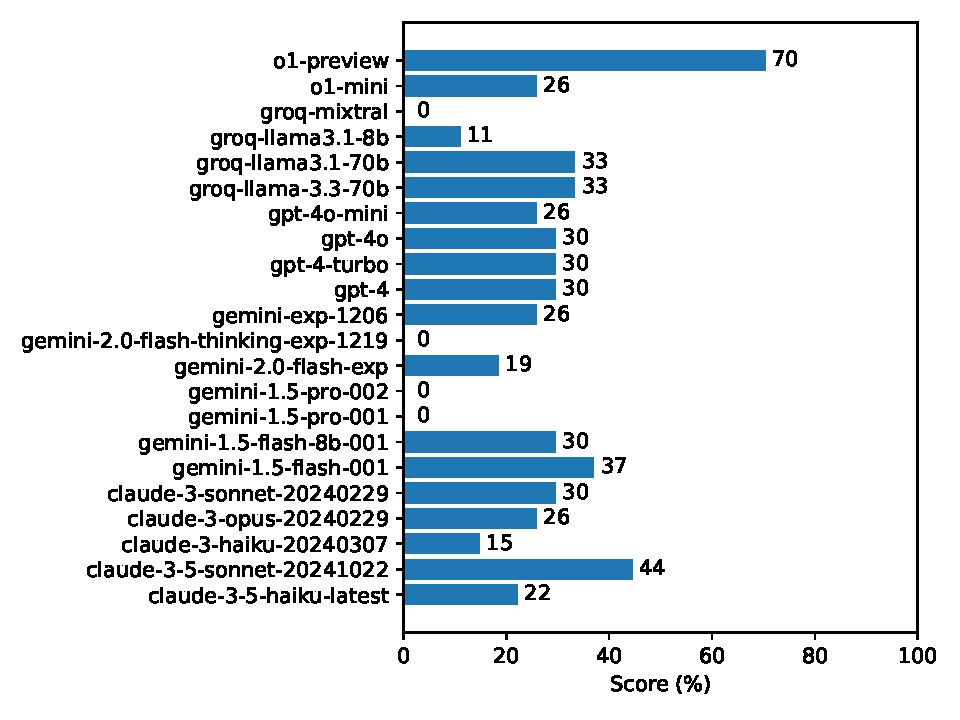
\includegraphics{llm_scores}
\end{document}